\documentclass[20pt]{beamer}
\usepackage[utf8]{inputenc}
\usepackage[T1]{fontenc}
\usepackage{lmodern}
\usepackage{graphicx}
\usetheme{default}


\newcommand\e{\emph}
\newcommand\tb{\textbf}
\newcommand\un{\underline}
\newcommand\txt{\texttt}


\begin{document}
	\author{Jennifer Lin}
	\title{Place of Residence and Political Attitudes in Democracies Worldwide}
	%\subtitle{}
	%\logo{}
	%\institute{New College of Florida}
	%\date{}
	%\subject{}
	\setbeamercovered{transparent}
	\setbeamertemplate{navigation symbols}{}
	\begin{frame}[plain]
	\maketitle
\end{frame}

\begin{frame}
\frametitle{Research Question}
\begin{enumerate}
	\item Does place of residence influence political attitudes and ideology? 
	\item How do certain factors of the regime, including its age and electoral formula, influence these results?
\end{enumerate}
\end{frame}

\begin{frame}
\begin{itemize}
\frametitle{Literature}
\item Case specifications 
\item Analysis of Polities
\end{itemize}
\end{frame}

\begin{frame}
\frametitle{The United States}
\begin{figure}[H]    \centering
	{	 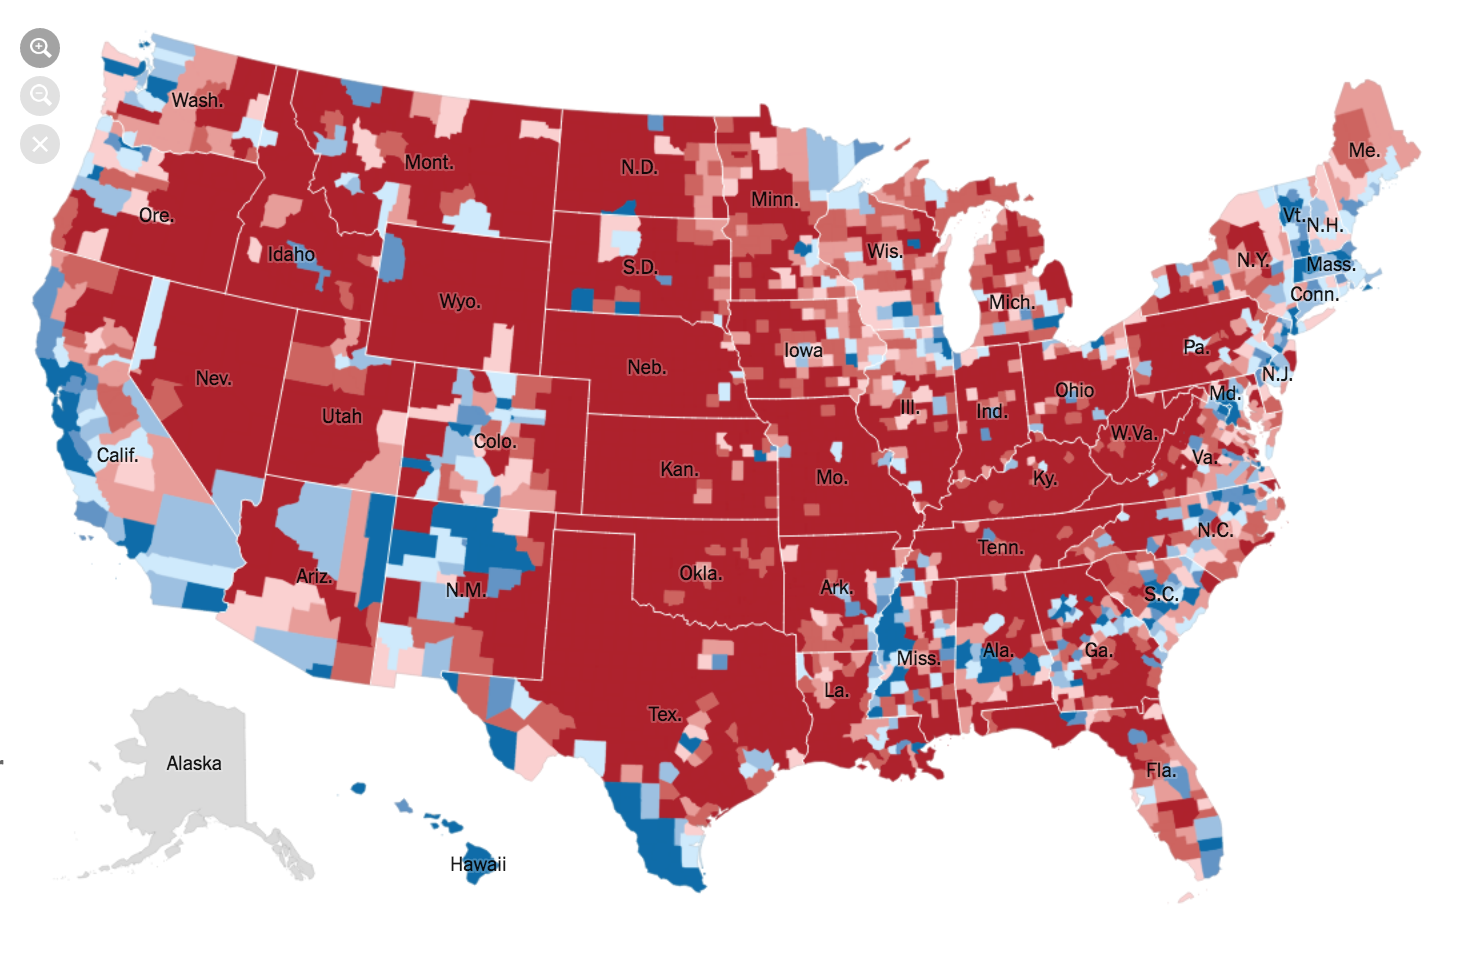
\includegraphics[width=\textwidth]{NYT}}
\end{figure}
\end{frame}

\begin{frame}
\frametitle{Polities in the CSES}
\begin{figure}[ht!]    \centering
	{	 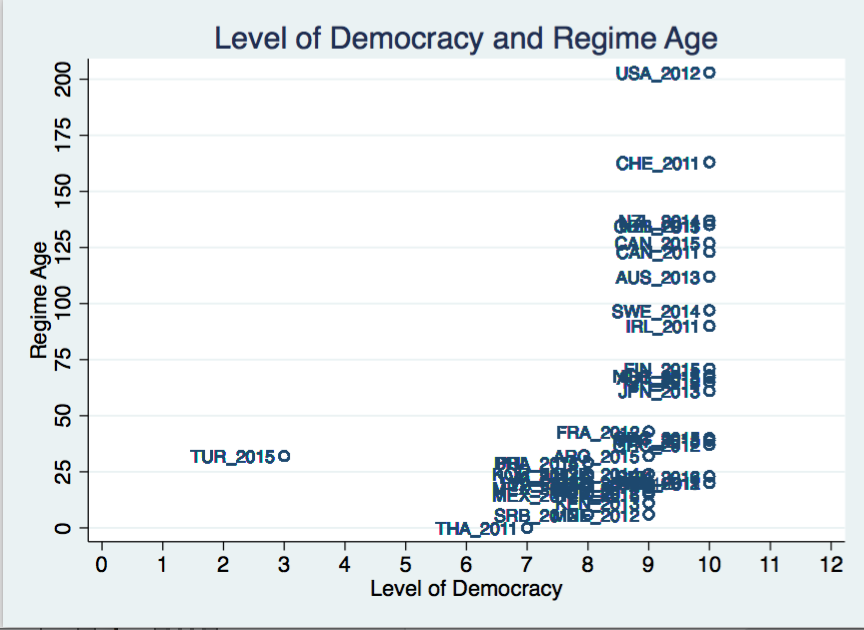
\includegraphics[width=.8\textwidth]{DemAge}}
\end{figure}
\end{frame}

\begingroup
\begin{frame}
\footnotesize
\frametitle{Hypotheses}
\e {Hypothesis 1 -- Place Matters} \\
~~\\
\e{Hypothesis 2 -- Issue Stances} \\
~~\\
\e{Hypothesis 3A -- Level of Democracy} \\
~~\\
\e{Hypothesis 3B -- Regime Age} \\
~~\\
\e{Hypothesis 3C -- Electoral Formula}\\
~~\\
\e{Hypothesis 3D -- Polity Differences} 

\end{frame}

\begin{frame}

\frametitle{Independent Measures}
\begin{itemize}
	\item Country
	\item Place of Residence
	\item Level of Democracy
	\item Regime Age
	\item Electoral Formula
\end{itemize}
\end{frame}

\begin{frame}

\frametitle{Dependent Measures}
\begin{itemize}
	\item Self-Placement Ideology (0-10)
	\item Liberalism - Public Expenditure and Income Inequality
\end{itemize}
\end{frame}

\begin{frame}

\frametitle{Results}
\begin{itemize}
	\item Self-Placement as Dependent Measure
	\item Liberalism as Dependent Measure
	\item Considerations of Macro Variables
\end{itemize}
\end{frame}

\begin{frame}
\frametitle{Conclusions}
When regressed on itself with regime variables, rural residents are significantly more conservative than urban residents - Yet, these points of conservatism are relatively small.
\end{frame}

\begin{frame}
\footnotesize
\frametitle{Hypotheses Revisited}

\e {Hypothesis 1 -- Place Matters} \\
~~\\
\e{Hypothesis 2 -- Issue Stances} \\
~~\\
\e{Hypothesis 3A -- Level of Democracy} \\
~~\\
\e{Hypothesis 3B -- Regime Age} \\
~~\\
\e{Hypothesis 3C -- Electoral Formula}\\
~~\\
\e{Hypothesis 3D -- Polity Differences} 

\end{frame}
\endgroup

\end{document}